\scanpage{229}
\mspage{762}

point $1$ de $\mathbb U$, de sorte que le rev. universel de
$\mathbb S_0$ pointé au dessus de $e_0$
s'identifie au \unsure{revêtement} exponentiel
\[
\tag{11}
\diagram{\begin{tikzcd}[ampersand replacement=\&,column sep=large,row sep=small]
\mathbb R \arrow[r] \& \mathbb U \&
(\xrightarrow{\sim}\mathbb S_0)\\
t \arrow[r,mapsto] \& \exp 2i\pi t \&
(\mapsto \mathbb R^+\exp 2i\pi t.
\end{tikzcd}}
\]

Ainsi, un relèvement de $u_{\unsure{\mathbb S^1}}$
\inserted{en $\widetilde u$} revient au choix de $t\in\mathbb R$ tel que
\[
\tag{12}
\exp 2i\pi t=\frac{u(1)}{|u(1)|}\qquad
\deleted{\unsure{\text{s'écr.}}}
\]
i.e. au choix d'un argument $t$ de $u(1)$.

On applique la construction de $\widetilde G$ du $1^\circ)$
au cas de $G=\mathrm{Gl}(2,\mathbb R)^{\pm1}$,
on trouve une structure d'extension
\[
\tag{13}
\diagram{\begin{tikzcd}[ampersand replacement=\&,column sep=1.4em]
1\arrow[r]\&\mathbb Z\arrow[r]\&
\mathrm{Gl}(2,\mathbb R)^{\pm1\,\sim}\arrow[r]\&
\mathrm{Gl}(2,\mathbb R)^{\pm1}\arrow[r]\&1.
\end{tikzcd}}
\]

\deleted{\unsure{Propo}}\inserted{qui induit}
au dessus de la composante neutre $\mathrm{Sl}(2,\mathbb R)$
de $\mathrm{Gl}(2,\mathbb R)^{\pm1}$ une structure d'extension
\[
\tag{14}
\diagram{\begin{tikzcd}[ampersand replacement=\&,column sep=1.5em]
1\arrow[r]\&\mathbb Z\arrow[r]\&
\mathrm{Sl}(2,\mathbb R)^{\sim}\arrow[r]\&
\mathrm{Sl}(2,\mathbb R)\arrow[r]\&1.
\end{tikzcd}}
\]

\begin{tabular}{|p{0.9\linewidth}}
\uline{Proposition} Le groupe $\mathrm{Sl}(2,\mathbb R)^{\sim}$ est
$1$-connexe, et $\overline{\mathrm m}$ \deleted{\unsure{contra}}
homéomorphe à $\mathbb R^3$.
\end{tabular}

\margin{228}

\begin{center}
228\\
\texttt{https://grothendieck.umontpellier.fr}\\
Université de Montpellier, UMR CNRS 5149, Case courrier 051, Place Eugène Bataillon\\
34095 Montpellier cedex 5 - France
\end{center}

\scanpage{230}

\uline{Dém.} Comme l'inclusion
\[
\tag{15}
\diagram{\begin{tikzcd}[ampersand replacement=\&,column sep=large]
\mathbb U\arrow[r,hook]\&\mathrm{Sl}(2,\mathbb R)
\end{tikzcd}}
\]
est une équivalence d'homotopie,
\deleted{\unsure{qui}} s'identifie \inserted{topologiquement}
à l'inclusion
$\diagram{\begin{tikzcd}[ampersand replacement=\&,column sep=large]
\mathbb U\arrow[r]\&\mathbb U\times\mathbb R^2
\end{tikzcd}}$,
on est ramené à prouver que
\deleted{\unsure{au dessus de} $\mathbb U$}
\inserted{l'image inverse $\mathbb U^{\sim}$}
de $\mathbb U$ dans $\mathrm{Sl}(2,\mathbb R)^{\sim}$
s'identifie au rev. universel
$\deleted{\unsure{\mathbb R}}\,\mathbb R$ de $\mathbb U$
(pointé au dessus de $1$ par $0\ldots$)
Or si $u\in\mathbb U$, le \deleted{\unsure{dernier}}
choix d'un $\widetilde u$ au dessus de $u$, i.e. d'un relèvement de
$\dfrac{u(1)}{|u(1)|}$ en $\mathbb R$ par la formule (12),
s'identifie (puisque $\dfrac{u(1)}{|u(1)|}=u(1)=u$)
au choix d'un $t\in\mathbb R$ tel que $\exp 2i\pi t\in u$, O.K.

\uline{Cor. 1} Le \unsure{sous-g.} \unsure{inv.} dans
$\mathrm{Sl}(\unsure{2},\mathbb R)^{\sim}$ d'un sous-groupe
cyclique fini \inserted{d'ordre $n$} est $\simeq\mathbb Z$
($\exists!$ générateur $\overline\omega$ de celui-ci,
tel qu'on ait $\overline\omega^{\,n}=\omega'_0$,
où $\omega'_0$ est le gén. \deleted{\unsure{can.}}
du $\operatorname{Ker}(\mathrm{Sl}(2,\mathbb R)^{\sim}
\to\mathrm{Sl}(2,\mathbb R))$).

\margin{En appliquant ceci au centre
$\{\pm1\}$ de $\mathrm{Sl}(2,\mathbb R)$,
on trouve un él. canonique $\omega_0\in\mathrm{Sl}(2,\mathbb R)^{\sim}$
avec $\omega_0^2=\omega'_0$.}

\uline{Cor. 2} L'action d'un $g\in\mathrm{Gl}(2,\mathbb R)^{-1}$
sur $\deleted{\unsure{\overline\omega}}\,\omega'_0$
(ou sur le centre $\omega_0^{\mathbb Z}$ de
$\mathrm{Sl}(2,\mathbb R)^{\sim}$)
est via $\omega'_0\mapsto{\omega'_0}^{-1}$
(resp. $\omega_0\mapsto\omega_0^{-1}$) $\ldots$

\margin{229}

\begin{center}
229\\
\texttt{https://grothendieck.umontpellier.fr}\\
Université de Montpellier, UMR CNRS 5149, Case courrier 051, Place Eugène Bataillon\\
34095 Montpellier cedex 5 - France
\end{center}

\scanpage{231}
\mspage{763}

$3^\circ)$ \uline{Le groupe} $\mathrm{Gl}(2,\mathbb Z)^{\sim}$.

Soit $\mathrm{Gl}(2,\mathbb Z)^{\sim}$ l'image inverse de
$\mathrm{Gl}(2,\mathbb Z)$ dans $\mathrm{Gl}(2,\mathbb R)^{\pm1\,\sim}$,
de sorte qu'on a une structure d'extension
\[
\tag{16}
\diagram{\begin{tikzcd}[ampersand replacement=\&,column sep=1.2em,row sep=small]
1\arrow[r]\&\mathbb Z\arrow[r]\&\mathrm{Gl}(2,\mathbb Z)^{\sim}\arrow[r]\&
\mathrm{Gl}(2,\mathbb Z)\arrow[r]\&1.\\
\&\deleted{\unsure{n}}\arrow[u,mapsto]\arrow[r,mapsto]\&
\deleted{\unsure{\omega'_0}}\\
\&n\arrow[r,mapsto]\&\unsure{\omega_0^n|{\omega'_0}^{\,n}}
\end{tikzcd}}
\]

Je voudrais décrire $\mathrm{Gl}(2,\mathbb Z)^{\sim}$ par générateurs
et relations. Pour ceci, je note ceci :

\begin{tabular}{|p{0.9\linewidth}}
\uline{Proposition} L'image inverse
\inserted{dans $\mathrm{Gl}(2,\mathbb Z)^{\sim}$}
des sous-groupes cycliques $L_\rho\simeq\mathbb Z/6\mathbb Z$
et $L_\sigma\simeq\mathbb Z/4\mathbb Z$ engendrés par
$\rho$ et $\sigma$ sont isomorphes à $\mathbb Z$.
\end{tabular}

Ceci résulte du

\uline{Corollaire} (à la prop. p. 762) : Pour tt sous-groupe
cyclique fini $\unsure{\mathfrak Z|\mathfrak z}\subset
\mathrm{Sl}(2,\mathbb R)$, l'image inverse de
$\unsure{\mathfrak Z|\mathfrak z}$ dans
$\mathrm{Sl}(2,\mathbb R)^{\sim}$ est isomorphe à $\mathbb Z$.

En effet, par conjugaison \unsure{SPS} que
$\unsure{\mathfrak Z|\mathfrak z}\subset\mathbb U$,
i.e. $\unsure{\mathfrak Z|\mathfrak z}=\mu_n(\mathbb C)$,
mais alors $\unsure{\widetilde{\mathfrak Z}|\widetilde{\mathfrak z}}$
s'identifie à l'ens des $t\in\mathbb R$ avec
$(\exp 2i\pi t)^n=1$ i.e. $\exp 2i\pi(nt)=1$ i.e.

\margin{230}

\begin{center}
230\\
\texttt{https://grothendieck.umontpellier.fr}\\
Université de Montpellier, UMR CNRS 5149, Case courrier 051, Place Eugène Bataillon\\
34095 Montpellier cedex 5 - France
\end{center}

\scanpage{232}

\[
t\in\frac1n\mathbb Z,
\]
le groupe de ces $t$ est $\simeq\mathbb Z$, cqfd.

\uline{Corollaire} Il existe
$\widetilde\rho\in\mathrm{Sl}(2,\mathbb Z)^{\sim}$ et
$\widetilde\sigma\in\mathrm{Sl}(2,\mathbb Z)^{\sim}$,
au dessus de $\rho$ et $\sigma$ respectivement, tels qu'on ait
\[
\tag{17}
\widetilde\rho^{\,3}=\widetilde\sigma^{-2}
\]
\margin{pour un énoncé plus \unsure{sympathique}, voir (20) plus bas $\ldots$}
L'ens de ces systèmes $(\widetilde\rho,\widetilde\sigma)$
est un torseur sous $\mathbb Z$, par l'opération
\[
\tag{18}
\diagram{\begin{tikzcd}[ampersand replacement=\&,column sep=large]
(\widetilde\rho,\widetilde\sigma)\arrow[r,mapsto]\&
(\widetilde\rho\,{\omega'_0}^{\,2n},
\widetilde\sigma\,{\omega'_0}^{\,3n}),
\end{tikzcd}}
\]
où $\omega'_0$ est le générateur canonique de
$\diagram{\begin{tikzcd}[ampersand replacement=\&,]
\mathrm{Sl}(2,\mathbb Z)^{\sim}\arrow[r]\&
\mathrm{Sl}(2,\mathbb Z)
\end{tikzcd}}$.

On peut dire aussi que l'image inverse de l'élément
$\deleted{\unsure{=-\mathrm{id}}}$
\inserted{du centre $\{\pm1\}$} de $\mathrm{Sl}(2,\mathbb Z)$
\deleted{\unsure{l'unique}}
\deleted{(l'élément central \unsure{distinct de|$\ne$}
$+1$ de $\mathrm{Sl}(2,\mathbb Z)$)}
\deleted{est un torseur sous $\mathbb Z$, et le choix}
\inserted{est un groupe isomorphe à $\mathbb Z$, avec un}
unique générateur $\omega_0$ satisfaisant
\deleted{\unsure{d'un} relèvement}
\[
\tag{19}
\begin{gathered}
\omega_0^2=\omega'_0
\quad(\inserted{\text{le}}\ \text{générateur can. de}\\
\diagram{\begin{tikzcd}[ampersand replacement=\&,]
\mathrm{Sl}(2,\mathbb Z)^{\sim}\arrow[r]\&
\mathrm{Sl}(2,\mathbb Z)
\end{tikzcd}})
\end{gathered}
\]

\margin{il \unsure{vaut} mieux dire : $\exists!$ gén.
$\widetilde\rho$ \inserted{(resp. $\widetilde\sigma$)}
de l'image inverse $\unsure{\widetilde L_\rho|L_\rho}$ de $L_\rho$
(resp. $L_\sigma$) dans $\mathrm{Sl}(2,\mathbb Z)^{\sim}$,
au dessus de $\rho$ (resp. $\sigma$), et on a alors les relations (20)}

et ceci étant, il est possible de relever $\rho$ en $\widetilde\rho$,
\inserted{$\sigma$ en $\widetilde\sigma$} satisfaisant
\[
\tag{20}
\widetilde\rho^{\,3}=\omega_0^{-1},\qquad
\widetilde\sigma^{\,2}=\omega_0
\]
\margin{\uline{Faire la vérification}}
Et cette fois-ci, $\widetilde\rho$ et $\widetilde\sigma$
sont uniquement déter-

\margin{231}

\begin{center}
231\\
\texttt{https://grothendieck.umontpellier.fr}\\
Université de Montpellier, UMR CNRS 5149, Case courrier 051, Place Eugène Bataillon\\
34095 Montpellier cedex 5 - France
\end{center}

\scanpage{233}
\mspage{764}

minés. Ceci résulte \deleted{\unsure{d'une façon}}
\inserted{\deleted{\unsure{de la}}}
aussitôt de la prop. précédente.

\unsure{i)} Considérons l'image inverse de $\{1,\tau\}\subset\mathrm{Gl}(2,\mathbb Z)$
dans $\mathrm{Gl}(2,\mathbb Z)^{\sim}$,
\deleted{\unsure{un gr.}} extension de
$\{1,\tau\}\simeq\mathbb Z/2\mathbb Z$ par $\mathbb Z$
--- je dis que cette extension est \uline{scindée}.

\margin{\uline{NB}
$\tau=\tau_\infty=\begin{pmatrix}-1&0\\0&1\end{pmatrix}$
i.e. $\tau(x+iy)=\unsure{-}x+iy$
(symétrie p.r. à l'axe des $y$)}

En effet, l'action de $\tau$ sur $\mathbb S_0$
se relève en l'action de $\widetilde\tau$ \deleted{de}
d'ordre $2$ sur
$\deleted{\unsure{\mathbb R}}\,
\widetilde{\mathbb S}_0\simeq\mathbb R$,
qui est donnée par
\[
\tag{21}
\widetilde\tau t=\frac12-t
\]
car on a pour $z\in\mathbb U$, $z=\exp 2i\pi t$
\[
\tag{22}
\begin{aligned}
\tau z&=-\overline z=-\exp 2i\pi t
=\exp(\pi it-2i\pi t)\\
&=\exp\unsure{\{}\,2i\pi
\underbrace{\left(\frac12-t\right)}_{\widetilde\tau(t)}.
\end{aligned}
\]

\deleted{Je} Il est peut-être plus commode de travailler avec
$\tau'=\tau'_\infty=\begin{pmatrix}0&1\\1&0\end{pmatrix}$,
qui \deleted{est} échange $e_0=1$ et $e_1=i$,
i.e. la symétrie \unsure{p.r.|par} à la diagonale principale.
Cet autom. stabilise $\mathbb U$, et fixe le pt
$\exp\dfrac{\pi i}{\unsure{4|8}}=\dfrac{\sqrt2}{2}(i+1)\unsure{)}$,
il se relève en
\[
\tag{23}
\widetilde{\tau'}(t)=2i\pi\left(\frac1{\unsure{8|4}}-t\right).
\]
Notons que \deleted{$\unsure{\widetilde{\tau'}|\tau'}$}
l'action de $\widetilde{\tau'}$ (comme celle

\margin{232}

\begin{center}
232\\
\texttt{https://grothendieck.umontpellier.fr}\\
Université de Montpellier, UMR CNRS 5149, Case courrier 051, Place Eugène Bataillon\\
34095 Montpellier cedex 5 - France
\end{center}

\scanpage{234}

de $\widetilde\tau$) sur $\omega_0$ est la symétrie $\omega_0\mapsto\omega_0^{-1}$ (cf fin du \S\ précédent). Je dis qu'on a
\[
\begin{array}{ll}
(24)&\widetilde\tau'(\widetilde\rho)=\widetilde\rho^{-1},\qquad
\widetilde\tau'(\widetilde\sigma)=\widetilde\sigma^{-1}.
\end{array}
\]
Les formules s'écrivent \unsure{aussi|ainsi}
\[
\widetilde\tau'(\widetilde\rho^{-1})=\widetilde\rho,\qquad
\widetilde\tau'(\widetilde\sigma^{-1})=\widetilde\sigma
\]
elles sont valables \deleted{\unsure{et}} dans $\unsure{\mathrm{Sl}}(2,\mathbb Z)$, donc pour voir qu'elles sont valables dans $\mathrm{Sl}(2,\mathbb Z)^{\sim}$, il suffit de montrer que les premiers \unsure{mbs} satisfont les relations \unsure{caractéristiques} (20), ce qui s'écrit
\[
\widetilde\tau'\bigl(\underbrace{\widetilde\rho^{-3}}_{\omega_0^{\deleted{\unsure{-1}}}}\bigr)=\omega_0^{-1},\qquad
\widetilde\tau'\bigl(\underbrace{\widetilde\sigma^{-2}}_{\omega_0^{-1}}\bigr)=\omega_0
\]
i.e. $\widetilde\tau'(\omega_0)=\omega_0^{-1}$, OK.

\begin{tabular}{|l}
\uline{Théorème.} Le groupe $\mathrm{Sl}(2,\mathbb Z)^{\sim}$ admet\\
la présentation (à deux gén. $\widetilde\rho,\widetilde\sigma$)\\[3pt]
$(25)\qquad\boxed{\widetilde\rho^3\cdot\widetilde\sigma^2=1}$
\end{tabular}

\uline{Dém.} Soit $\unsure{\Pi|\pi}$ le groupe \deleted{\unsure{engendré}} \inserted{défini} par cette présentation, et considérons l'hom
\diagram{
\begin{tikzcd}[ampersand replacement=\&,column sep=large,row sep=tiny]
\unsure{\Pi|\pi}\arrow[r] \& \mathrm{Sl}(2,\mathbb Z)/\pm1=\{\rho,\sigma\mid\rho^3=\sigma^2=1\}\\
(\widetilde\rho,\widetilde\sigma)\arrow[r,mapsto] \& (\rho,\sigma)\ \mathrm{mod}\{\pm1\}
\end{tikzcd}
\quad(26)
}

\margin{233}

\begin{center}
233\\
\texttt{https://grothendieck.umontpellier.fr}\\
Université de Montpellier, UMR CNRS 5149, Case courrier 051, Place Eugène Bataillon\\
34095 Montpellier cedex 5 - France
\end{center}

\scanpage{235}
\mspage{765}

le groupe $\mathrm{Sl}(2,\mathbb Z)/\pm1$ s'identifie au quotient de $\unsure{\pi|\Pi}$ par le sous-groupe distingué engendré par l'élément $\uline{\omega_0}\overset{\mathrm{dfn}}{=}\widetilde\rho^{-3}=\widetilde\sigma^2$.
Mais cet élément étant \unsure{central}, le groupe engendré par $\uline{\omega_0}$ est déjà distingué.
donc on a une suite exacte
\diagram{
$(27)\quad$
\begin{tikzcd}[ampersand replacement=\&,column sep=large,row sep=tiny]
n\arrow[r,mapsto] \& \uline{\omega_0}^{n} \& \& \\
\mathbb Z\arrow[r] \& \unsure{\Pi|\pi}\arrow[r] \& \mathrm{Sl}(2,\mathbb Z)/\pm1\arrow[r] \& 1
\end{tikzcd}
}
qui s'envoie dans la suite exacte
\diagram{
\deleted{$\unsure{(28)|(27)}$}\quad
\begin{tikzcd}[ampersand replacement=\&,column sep=large,row sep=tiny]
1\arrow[r] \& \mathbb Z\arrow[r] \& \mathrm{Sl}(2,\mathbb Z)^{\sim}\arrow[r] \& \mathrm{Sl}(2,\mathbb Z)/\pm1\arrow[r] \&1\\
\& n\arrow[r,mapsto] \&\omega_0^{n}\&\&
\end{tikzcd}
}
en induisant des iso \inserted{identiques} sur les facteurs extrêmes --- donc par le lemme \unsure{des|de} $5$
$\unsure{\pi|\Pi}\longrightarrow\mathrm{Sl}(2,\mathbb Z)^{\sim}$ est iso, cqfd.

\begin{tabular}{|l}
\uline{Corollaire 1} Le groupe $\mathrm{Gl}(2,\mathbb Z)^{\sim}$ admet\\
la présentation (à trois gén. $\widetilde\rho,\widetilde\sigma,\widetilde\tau'$)
\end{tabular}
\[
\begin{array}{ll}
(28)&\boxed{
\widetilde\tau'{}^{2}=\deleted{\unsure{1,|\omega_0}}\,
\widetilde\rho^3\cdot\widetilde\sigma^2=1,\quad
\widetilde\tau'(\widetilde\rho)=\widetilde\rho^{-1},\quad
\widetilde\tau'(\widetilde\sigma)=\widetilde\sigma^{-1}}
\end{array}
\]

Je vais \unsure{essayer} de présenter le \deleted{\unsure{élément}} \inserted{groupe}
$\mathrm{Gl}(2,\mathbb Z)^{\sim}$ \unsure{avec|en} trois générateurs involutifs,
\deleted{\unsure{au de}} $\widetilde r_0,\widetilde r_1,\widetilde r_\infty$ au dessus des éléments
$r_0,\unsure{r_1|\sigma_0},r_\infty$ de $\mathrm{Gl}(2,\mathbb Z)^{-}$, en \unsure{m'inspirant} \unsure{du formulaire|des formulaires} de $\mathrm{Sl}(2,\mathbb Z)$ :

\margin{234}

\begin{center}
234\\
\texttt{https://grothendieck.umontpellier.fr}\\
Université de Montpellier, UMR CNRS 5149, Case courrier 051, Place Eugène Bataillon\\
34095 Montpellier cedex 5 - France
\end{center}

\scanpage{236}

\[
\begin{array}{ll}
(29)&\left\{
\begin{aligned}
r_\infty&=\tau_\infty=\begin{pmatrix}-1&0\\0&1\end{pmatrix}\\
r_0&=\tau'_\infty=\begin{pmatrix}0&1\\1&0\end{pmatrix}\\
r_1&=-\tau'_0=\begin{pmatrix}-1&1\\0&1\end{pmatrix}
\end{aligned}
\right.
\end{array}
\]
\margin{$\left[\begin{array}{ll}
(30)&\left\{
\begin{aligned}
r_0(\rho)&=\rho^{-1},\quad r_0(\sigma)=\sigma^{-1}\\
r_1&=\rho^{-1}r_0=r_0\rho\\
r_\infty&=\sigma r_0=r_0\sigma^{-1}
\end{aligned}\right.
\end{array}\right.$}

Notons que $(\widetilde\rho,\widetilde\tau')$ \unsure{engendrent} un groupe isomorphe à $D_\infty$, que je note $D_{\widetilde\rho}$,
de $\overline{\mathrm m}$ $(\widetilde\sigma,\widetilde\tau')$ \unsure{engendre|engendrent} un groupe $D_{\widetilde\sigma}$,
isomorphe à $D_\infty$. Enfin $(\omega_0,\widetilde\tau')$ \unsure{engendrent} un groupe $D_{\omega_0}$, isomorphe encore à $D_\infty$. On a un diagramme
\diagram{
$(31)\quad$
\begin{tikzcd}[ampersand replacement=\&,column sep=large,row sep=large]
\&D_{\omega_0}\arrow[dl,"i"']\arrow[dr,"j"]\&\\
D_{\widetilde\rho}\&\&D_{\unsure{\widetilde\sigma|\widetilde\rho}}
\end{tikzcd}
\qquad
$\begin{aligned}
&\left\{\begin{aligned}
i(\omega_0)&=\widetilde\rho^{-3}\\
i(\widetilde\tau')&=\widetilde\tau'
\end{aligned}\right.\\[4pt]
&\left\{\begin{aligned}
j(\omega_0)&=\widetilde\sigma^2\\
j(\unsure{\widetilde\tau'})&=\widetilde\tau'
\end{aligned}\right.
\end{aligned}$
}
et le cor. 1 s'écrit sous la forme
\[
\begin{array}{ll}
(32)&\mathrm{Gl}(2,\mathbb Z)^{\sim}\simeq D_{\widetilde\rho}*_{D_{\omega_0}}D_{\widetilde\sigma}
\end{array}
\]
(\unsure{somme} amalgamée de groupes).

Or on peut prendre dans $D_{\widetilde\rho},D_{\widetilde\sigma}$ les générateurs involutifs
\[
\begin{array}{ll}
(33)&\left\{\begin{array}{lll}
\widetilde r_0=\widetilde\tau'=\widetilde\tau'_\infty&\text{et}&
\widetilde r_1\overset{\mathrm{dfn}}{=}\widetilde\rho^{-1}\widetilde r_0=\widetilde r_0\widetilde\rho\quad\text{dans }D_{\widetilde\rho}\\
\widetilde r_0=\cdots\cdots&\text{et}&
\widetilde r_\infty\overset{\mathrm{dfn}}{=}\unsure{\widetilde\sigma\,\widetilde r_0}=\widetilde r_0\widetilde\sigma^{-1}
\end{array}\right.
\end{array}
\]

\margin{235}

\begin{center}
235\\
\texttt{https://grothendieck.umontpellier.fr}\\
Université de Montpellier, UMR CNRS 5149, Case courrier 051, Place Eugène Bataillon\\
34095 Montpellier cedex 5 - France
\end{center}

\scanpage{237}
\mspage{766}

et on trouve alors

\uline{Corollaire 2} $\mathrm{Gl}(2,\mathbb Z)^{\sim}$ admet une présentation (à trois générateurs involutifs $\widetilde r_0,\widetilde r_1,\widetilde r_\infty$) :
\[
\begin{array}{ll}
(34)&\boxed{\widetilde r_0^2=\widetilde r_1^2=\widetilde r_\infty^2=1,\quad
\Bigl(\underbrace{\widetilde r_0^{\deleted{\unsure{-1}}}\widetilde r_1}_{\widetilde\rho}\Bigr)^3
\overset{\deleted{\unsure{=}}}{\cdot}
\Bigl(\underbrace{\widetilde r_\infty\widetilde r_0^{\deleted{\unsure{-1}}}}_{\widetilde\sigma}\Bigr)^2=1}\\[-2pt]
&\hspace{13em}\deleted{\underbrace{\hspace{9em}}_{\unsure{\omega_0}}}
\end{array}
\]

\margin{236}

\begin{center}
236\\
\texttt{https://grothendieck.umontpellier.fr}\\
Université de Montpellier, UMR CNRS 5149, Case courrier 051, Place Eugène Bataillon\\
34095 Montpellier cedex 5 - France
\end{center}

\scanpage{238}

$4^\circ)$ \uline{L'isomorphisme} $\mathrm{Gl}(2,\mathbb Z)^{\sim}\simeq S\mathcal T_{1,1}$

\margin{$\unsure{\checkmark}$}
Posons
\[
\begin{array}{ll}
(35)&\deleted{\unsure{X_1}}\quad X_1=\mathbb R^2/\mathbb Z^2\simeq(\mathbb R/\mathbb Z)^2\simeq\mathbb U\times\mathbb U.
\end{array}
\]
(surface-type de genre $1$), notons additivement sa loi de composition, et soit
\[
\begin{array}{ll}
(36)&a_{1,0}=0\in X_1,\quad X_1\setminus\{a_{1,0}\}=X_1\setminus\{0\}=U_{1,1},
\end{array}
\]
surface-type de type $(g,\nu)=(1,1)$.

Le groupe $\mathrm{Gl}(2,\mathbb Z)$ s'identifie au groupe des automorphismes du groupe topologique $X_1$, et opère donc sur $X_1$ en laissant fixe l'origine $\deleted{a_{1,0}}\ 0$, donc il opère sur $U_{1,0}$, d'où un hom
\diagram{
$(37)\quad$
\begin{tikzcd}[ampersand replacement=\&,column sep=large,row sep=tiny]
\mathrm{Gl}(2,\mathbb Z)\arrow[r,"\sim"]\&\mathcal T_{1,1}=\mathcal T(\unsure{U_{1,1}})\\
\&\begin{gathered}\text{groupe des classes d'isotopie}\\
\text{d'homéomorphismes}\\
\text{de }U_{1,1},\end{gathered}
\end{tikzcd}
}
dont on sait que c'est un isomorphisme. D'ailleurs, $G=\mathrm{Gl}(2,\mathbb Z)$ opère \unsure{différentiablement|différentiellement} sur $\deleted{\unsure{\mathcal T|\tau}}\ X_1$, et l'action sur l'espace \uline{tangent} s'identifie à l'action tautologique de $\mathrm{Gl}(2,\mathbb Z)\subset\mathrm{Gl}(2,\mathbb R)$ sur $\mathbb R^2$. Donc le groupe noté $\widetilde G$ dans

\margin{237}

\begin{center}
237\\
\texttt{https://grothendieck.umontpellier.fr}\\
Université de Montpellier, UMR CNRS 5149, Case courrier 051, Place Eugène Bataillon\\
34095 Montpellier cedex 5 - France
\end{center}

\scanpage{239}
\mspage{767}

\unsure{$1^\circ$)} \unsure{e} est canoniquement isomorphe, en tant qu'extension de $G$ par $T_0=\mathbb Z$ (NB. $\mathbb R^2$ et son quotient $X_1$ sont canoniquement orientés) au groupe $\mathrm{Gl}(2,\mathbb Z)^\sim$ \unsure{du} $3^\circ$.

Ainsi on trouve \deleted{le \unsure{Théorème}} \inserted{(cf. prop. p. 761)} le

\uline{Théorème} L'image inverse par l'isom. (37) de l'extension $S\deleted{\unsure{*}}\mathcal T_{1,1}$ de $\mathcal T_{1,1}$ par $\mathbb Z$ s'identifie canoniquement à $\mathrm{Gl}(2,\mathbb Z)^\sim$, donc il admet les \inserted{deux} présentations explicites \unsure{du} $3^\circ$
\[
\begin{aligned}
\text{a)}\quad &
\underset{\deleted{\unsure{\omega\widetilde\sigma}}}{\widetilde\rho^{3}\cdot\widetilde\sigma^{2}}
=\underset{\deleted{\unsure{\omega_0}}}{1},\quad
\unsure{\widetilde\tau'}(\widetilde\rho)=\widetilde\rho^{-1},\quad
\widetilde\tau'(\widetilde\sigma)=\widetilde\sigma^{-1},\quad
\widetilde\tau'^{\,2}=1
\\[1ex]
\text{b)}\quad &
\widetilde r_0^{2}=\widetilde r_1^{2}=\widetilde r_\infty^{2}=1,\quad
\underset{\deleted{\unsure{\omega_0}}}{
(\widetilde r_0^{\deleted{\unsure{-1}}}\widetilde r_1)^3\cdot
(\widetilde r_\infty\widetilde r_0)^2}=1.
\end{aligned}
\]

Interprétons maintenant $\mathcal T_{1,1}$ et $S\mathcal T_{1,1}$ en termes du groupe fondamental de $U_{1,1}$, que nous \unsure{calculerons} en choisissant (judicieusement ?) un pt base $a_{1,1}$ dans $U_{1,1}$,
\[
\text{(38)}\qquad
\Pi_{1,1}\overset{\mathrm{dfn}}=\pi_1(U_{1,1},a_{1,1}),
\]
\[
\text{(39)}\qquad
\mathcal T_{1,1}\simeq\mathrm{Aut\,ext}_{\mathrm{lac}}(\Pi_{1,1})
\]
\margin{238}

\begin{center}
238\\
\texttt{https://grothendieck.umontpellier.fr}\\
Université de Montpellier, UMR CNRS 5149, Case courrier 051, Place Eugène Bataillon\\
34095 Montpellier cedex 5 - France
\end{center}

\scanpage{240}

\margin{\unsure{j'utilise} la \unsure{not.} $\ell'_0$ au lieu de $\ell_0$, car $\ell_0$ désigne déjà un élément bien déterminé de $\mathrm{Gl}(2,\mathbb Z)$ !}

Nous avons une présentation de $\Pi_{1,1}$ par
\[
\text{(40)}\qquad
\Pi_{1,1}=\{x,y,\ell'_0\mid [x,y]\ell'_0=1\}
\]
et désignant par $L$ le sous-groupe\inserted{\unsure{-lacets}} de $\Pi_{1,1}$ engendré par $\ell'_0$, on aura
\[
\text{(41)}\qquad
S\mathcal T_{1,1}\simeq
\mathrm{Norm}_{\mathrm{Aut}_{\mathrm{lac}}(\Pi_{1,1})}(L).
\]

Donc il faudrait expliciter l'action
\deleted{\unsure{de} $\unsure{S}$}
\diagram{\begin{tikzcd}[ampersand replacement=\&,column sep=large]
S\mathcal T_{1,1}\simeq\mathrm{Gl}(2,\mathbb Z)^\sim
\arrow[r] \& \mathrm{Aut}_{\mathrm{lac}}(\Pi_{1,1}),
\end{tikzcd}}
par l'action des générateurs $\widetilde\rho,\widetilde\sigma,\widetilde\tau'$ ou $\widetilde r_0=\widetilde\tau',\widetilde r_1,\widetilde r_\infty$ --- action qui doit \unsure{normaliser} $L$, et de façon plus précise, transformer $\ell'_0$ en $\ell'_0$ (pour $\widetilde\rho,\widetilde\sigma$) ou en $\ell_0'^{-1}$ (pour $\widetilde\tau'=\widetilde r_0,\widetilde r_1,\widetilde r_\infty$). Il faut donc expliciter l'action des générateurs sur $x$ et sur $y$. (NB $\Pi_{1,1}$ est le groupe libre ayant comme générateurs $x$ et $y$ \unsure{!})

Considérons le revêtement principal $U_{1,1}^{\prime\,\unsure{a}}$ de groupe $\mathbb Z^2$ de $U_{1,1}=X_1-\{0\}$, induit par le \unsure{rev.} principal $\mathbb R^2$ de $X_1=\mathbb R^2/\mathbb Z^2$, --- l'image inverse de $U_{1,1}$ est $\mathbb R^2\setminus\mathbb Z^2$. Choisissons un pt base \deleted{$\unsure{a}$}
\margin{239}

\begin{center}
239\\
\texttt{https://grothendieck.umontpellier.fr}\\
Université de Montpellier, UMR CNRS 5149, Case courrier 051, Place Eugène Bataillon\\
34095 Montpellier cedex 5 - France
\end{center}

\scanpage{241}
\mspage{768}

\deleted{\unsure{(44)|(42)}}
\[
a\in\mathbb R^2\setminus\mathbb Z^2,
\]
\unsure{au} dessus de $a_{1,1}$, on aura donc un iso. can.
\[
\text{(42)}\qquad
\Pi_{1,1}\simeq\pi_1(\mathbb R^2\setminus\mathbb Z^2,\mathbb Z^2;a)
\]
d'où une suite exacte
\diagram{\begin{tikzcd}[ampersand replacement=\&,column sep=small,row sep=small]
\text{(43)}\quad \& 1\arrow[r] \&
\pi_1(\mathbb R^2\setminus\mathbb Z^2)\arrow[r] \&
\Pi_{1,1}\arrow[r]\arrow[d,equal] \&
\mathbb Z^2\arrow[r]\arrow[d,phantom,"\simeq"{description,rotate=90}] \& 1.\\
\&\&\&\pi_1(U_{1,1}=X_1\setminus\{a_{1,0}\}) \&
\pi_1(X_1)\arrow[d,phantom,"\simeq"{description,rotate=90}] \&\\
\&\&\&\& (\Pi_{1,1})_{\mathrm{ab}} \&
\end{tikzcd}}

Les éléments du $\pi_1$ mixte s'explicitent par le calcul de Jean Malgoire à l'aide des couples
\[
\text{(44)}\qquad
(\gamma,\ell)\qquad
\left(\begin{gathered}
\gamma\in\mathbb Z^2,\quad \ell\ \text{\unsure{classe} de chemins dans}\\
\mathbb R^2\setminus\mathbb Z^2\ \text{de }a\text{ à }\deleted{\unsure{\gamma|\tau}}a+\gamma
\end{gathered}\right)
\]
qu'on ``\unsure{compose} comme les fonctions''.

\inserted{Nous prendrons, au dessus des générateurs}
\deleted{Considérons les}
$e_0,e_1$ de $\mathbb Z^2$, les éléments $x,y$ définis par les chemins rectilignes de $a$ à $a+e_0$, resp. $a+e_1$, à partir de l'origine
\[
\text{(45)}\qquad
 a=\widetilde a_{1,1}=\left(+\frac12,+\frac12\right)
\]

\figure{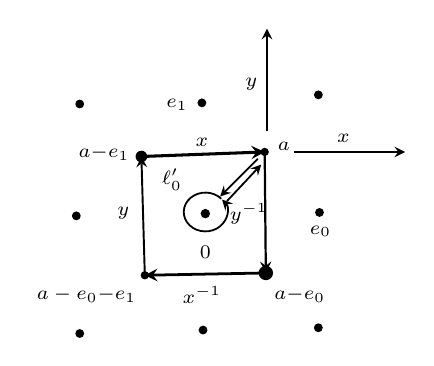
\begin{tikzpicture}[x=1.45cm,y=1.45cm,>=stealth,font=\scriptsize]
\fill (-1.10,0.96) circle (1.6pt);
\fill (-0.03,0.97) circle (1.6pt);
\fill (0.99,1.04) circle (1.6pt);
\fill (-1.13,-0.02) circle (1.6pt);
\fill (0,0) circle (1.7pt);
\fill (1.00,0.01) circle (1.6pt);
\fill (-1.10,-1.05) circle (1.6pt);
\fill (-0.02,-1.02) circle (1.6pt);
\fill (0.99,-1.00) circle (1.6pt);
\node[left] at (-0.07,0.95) {$e_1$};
\node[below] at (1.01,-0.02) {$e_0$};
\node[below] at (0,-0.20) {$0$};
\coordinate (a) at (0.52,0.54);
\coordinate (b) at (-0.56,0.50);
\coordinate (c) at (-0.53,-0.54);
\coordinate (d) at (0.53,-0.52);
\fill (a) circle (1.5pt);
\fill (b) circle (2.1pt);
\fill (c) circle (1.5pt);
\fill (d) circle (2.6pt);
\draw[->,line width=1.1pt] (b) -- (a);
\node[above] at (-0.03,0.50) {$x$};
\draw[->,line width=.7pt] (c) -- (b);
\node[left] at (-0.58,0.00) {$y$};
\draw[->,line width=1.0pt] (d) -- (c);
\node[below] at (-0.03,-0.55) {$x^{-1}$};
\draw[->,line width=.8pt] (a) -- (d);
\node at (0.38,0.00) {$y^{-1}$};
\draw[->,line width=.7pt] (0.54,0.72) -- (0.54,1.62);
\node[left] at (0.54,1.13) {$y$};
\draw[->,line width=.7pt] (0.78,0.54) -- (1.75,0.54);
\node[above] at (1.21,0.54) {$x$};
\node[right] at (0.55,0.59) {$a$};
\node[left] at (-0.58,0.53) {$a\unsure{-}e_1$};
\node[below left] at (-0.52,-0.56) {$a-e_0\unsure{-}e_1$};
\node[below right] at (0.52,-0.56) {$a\unsure{-}e_0$};
\draw[->,line width=.65pt] (0.46,0.48) -- (0.13,0.15);
\draw[->,line width=.65pt] (0.19,0.11) -- (0.49,0.43);
\draw[->,line width=.65pt] (0.14,0.13)
 arc[start angle=43,end angle=400,x radius=.19,y radius=.17];
\node[above left] at (-0.12,0.12) {$\ell'_0$};
\end{tikzpicture}}

Alors l'élément $xyx^{-1}y^{-1}$ est figuré par le chemin ci-dessus, qui est visiblement opposé au lacet ``rectiligne'' direct de $a$ autour de l'origine $0$.
\margin{240}

\begin{center}
240\\
\texttt{https://grothendieck.umontpellier.fr}\\
Université de Montpellier, UMR CNRS 5149, Case courrier 051, Place Eugène Bataillon\\
34095 Montpellier cedex 5 - France
\end{center}

\scanpage{242}

$5^\circ$) \uline{Digression sur les} \inserted{\uline{revêtements de}} \uline{germes d'espaces.}

\margin{A) \uline{Revêtements de germes}}
\margin{ici on n'exclut \deleted{\unsure{le}} \inserted{pas le} filtre impropre $(\varnothing\in\Phi)$ correspondant au germe d'espace \uline{vide}}

Un ``germe d'espace'' est défini par un espace topologique $S$ et une \deleted{base de} filtre $\Phi$ sur $S$, un morphisme de $(S,\Phi)$ dans $(S',\Phi')$ est un élément de
\[
\text{(46)}\qquad
\varinjlim_{S_i\in\Phi}\operatorname{Hom}_{\Phi_{\unsure{S_i|S'_i}},\Phi'}(S_i,S'),
\]
où \deleted{$\Phi_{S_i}$ est} pour $S_i\in\Phi$, $\Phi_{S_i}$ est le filtre induit par $\Phi$ sur $S_i$, et $\operatorname{Hom}_{\Phi_{S_i},\Phi'}$ désigne l'ensemble des appl. continues \inserted{$f$} de $S_i$ dans $S'$ compatibles avec $\Phi_{S_i},\Phi'$, i.e. telles que $\forall S'_j\in\Phi'$, \deleted{$\unsure{f}$} on ait $f^{-1}(S'_j)\in\Phi_{S_i}$. La composition des morphismes de germes est évidente.

Un \uline{revêtement} (étale) d'un germe $(S,\Phi)$ d'espaces top. est un objet de la catégorie
\[
\text{(47)}\qquad
\underline{\mathrm{Rev}}(S,\Phi)=\varinjlim_{S_i\in\Phi}\underline{\mathrm{Rev}}(S_i);\qquad\unsure{*}
\]
\unsure{ces|les} revêtements forment une catégorie, que nous pourrions \inserted{sans doute} interpréter \inserted{(au moins dans des ``bons cas'')} comme la catégorie des revêtements d'un topos convenable (savoir le topos limite
\margin{241}

\begin{center}
241\\
\texttt{https://grothendieck.umontpellier.fr}\\
Université de Montpellier, UMR CNRS 5149, Case courrier 051, Place Eugène Bataillon\\
34095 Montpellier cedex 5 - France
\end{center}

\scanpage{243}
\mspage{769}

\margin{cela \unsure{a été} fait par Olivier Leroy ?}

projective des \inserted{(petits)} topos étales des $S_i\in\Phi$).

Cette catégorie, ``dans les bons cas'', a tendance à être multigaloisienne, voire galoisienne.

On dit qu'un germe \deleted{\unsure{est}} d'espaces est $1$-connexe, ou simplement connexe, si le foncteur naturel

\diagram{\begin{tikzcd}[ampersand replacement=\&,column sep=large,row sep=small]
{(48)} \& (\mathrm{Ens}) \arrow[r] \& \underline{\mathrm{Rev}}(S,\Phi) \\
 \& E \arrow[r,mapsto] \& {\unsure{{}^{1}\!E_{(S,\Phi)}|\widetilde E_{(S,\Phi)}},\ \text{rev. const. de}} \\
 \& \& {\text{valeur }\unsure{E|\Phi}}
\end{tikzcd}}

est une équivalence de catégories. Ceci signifie que

$1^\circ)$ Ce foncteur est pl. fidèle (on dit que $(S,\Phi)$ est $0$-connexe), ce qui signifie, si $S$ est loc. connexe, que $\forall S_i\in\Phi$, $\exists S_j\in\Phi$, $S_j\subset S_i$, tel que \inserted{$S_j\ne\varnothing$ et} $(\pi_0(S_j)\longrightarrow\pi_0(S_i))$ soit une application constante

\margin{donc ceci implique que ce germe d'espaces est non vide}

$2^\circ)$ le foncteur est de plus \unsure{ess!|ess$^{\mathrm t}$} surjectif, ce qui signifie que pour tout $S_i\in\Phi$, $\exists S_j\in\Phi$, \inserted{$S_j\subset S_i$} tel que pour tte composante connexe $S_{j,\alpha}$ de $S_j$, l'hom. ext. $\pi_1(S_{j,\alpha})\longrightarrow\pi_1(S_i)$ soit trivial.

Les revêtements de germes d'espaces forment une catégorie fibrée sur celle

\margin{242}

\begin{center}
242\\
\texttt{https://grothendieck.umontpellier.fr}\\
Université de Montpellier, UMR CNRS 5149, Case courrier 051, Place Eugène Bataillon\\
34095 Montpellier cedex 5 - France
\end{center}

\scanpage{244}

des germes d'espaces. La catégorie des espaces top. \deleted{\illegible{1}} peut être considérée comme sous-catégorie pleine de celle des germes d'espaces topologiques en \unsure{associant} à tt espace $\unsure{S}$, le germe $(S,\Phi)$, où $\Phi$ est le filtre trivial sur $S$. Ceci étant, la cat. fibrée des revêtements de germes d'espaces \unsure{induit|induite} celle des rev. d'espaces topologiques.

Soit $\deleted{\unsure{\mathcal S}}\mathcal X$ un germe d'espaces tel que $\underline{\mathrm{Rev}}\mathcal X$ soit une catégorie \inserted{multi}galoisienne, \deleted{Alors} et soit $\mathcal S$ un germe d'espaces $1$-connexe, $\mathcal S\longrightarrow\mathcal X$ un morphisme. Alors on a

\diagram{\begin{tikzcd}[ampersand replacement=\&,column sep=large]
{(49)} \& \underline{\mathrm{Rev}}(\mathcal X) \arrow[r] \& \underline{\mathrm{Rev}}(\mathcal S) \& (\mathrm{Ens}) \arrow[l,"\sim"']
\end{tikzcd}}

foncteur fibre sur $\underline{\mathrm{Rev}}(\mathcal X)$, ce qui permet de définir
\[
(50)\qquad \pi_1(\deleted{\unsure{\mathcal S}}\unsure{\mathcal X},\mathcal S)
\]
comme le $\pi_1$ relatif à ce foncteur fibre. Si $\mathcal X$ est $0$-connexe donc $\underline{\mathrm{Rev}}(\mathcal X)$ est galoisienne, on aura donc, si $\Pi\simeq\pi_1(\mathcal X,\mathcal S)$, une équivalence de catégories

\margin{243}

\begin{center}
243\\
\texttt{https://grothendieck.umontpellier.fr}\\
Université de Montpellier, UMR CNRS 5149, Case courrier 051, Place Eugène Bataillon\\
34095 Montpellier cedex 5 - France
\end{center}

\scanpage{245}
\mspage{770}

\[
(51)\qquad \underline{\mathrm{Rev}}(\mathcal X)\simeq\mathrm{Ens}(\Pi).
\]

Le groupe $\pi_1(\mathcal X,\mathcal S)$ dépend fonctoriellement du triple $(\mathcal S,\mathcal X,\mathcal S\longrightarrow\mathcal X)$ i.e de la flèche $\mathcal S\longrightarrow\mathcal X$ dans la catégorie des germes d'espaces, où $\deleted{\mathcal S}$ la source $\mathcal S$ est $1$-connexe.

\unsure{Soient|Soit} $X$ un espace top., $Y$ une partie de $X$, on \uline{appelle germe de} $X$ \uline{autour de} $Y$ le germe d'espaces $(X,\Phi)$, où $\Phi$ est le filtre des voisinages de $Y$ \unsure{dans|ds} $X$, \uline{germe résiduel de $X$ autour de $Y$} le germe d'espaces $(X\setminus Y,\Phi_{X\setminus Y})$ induit sur $X-Y$ (il est vide ssi $Y$ est ouvert).

\margin{On a un \unsure{diagramme} de morphismes \unsure{canoniques}
\diagram{\begin{tikzcd}[ampersand replacement=\&,column sep=large,row sep=large]
\unsure{\mathrm{Germ}_{Y}(X)} \arrow[d,hook] \& \unsure{\mathrm{Gerres}_{Y}(X)} \arrow[l,hook'] \arrow[d,hook] \\
X \& X-Y \arrow[l,hook']
\end{tikzcd}}\quad (52)}

Nous utiliserons cette notion \deleted{\unsure{surtout}} dans le cas où $Y=\{x\}$, en parlant aussi de germe et germe résiduel de $X$ en $x$. (\uline{NB} le germe de $X$ en $x$ est tjrs \deleted{\unsure{simp}} $1$-connexe, mais pas le germe résiduel). Tout germe d'espaces \inserted{$(S,\Phi)$} peut s'interpréter comme germe résiduel d'un espace \deleted{$(\unsure{S},\unsure{\Phi})$} $\unsure{X}=S\cup\{\omega\}$ en un pt $\omega$ convenable \ldots

\margin{244}

\begin{center}
244\\
\texttt{https://grothendieck.umontpellier.fr}\\
Université de Montpellier, UMR CNRS 5149, Case courrier 051, Place Eugène Bataillon\\
34095 Montpellier cedex 5 - France
\end{center}

\scanpage{246}

\unsure{.} Je m'intéresse au cas où $x\in X$ admet un voisinage homéomorphe à $\mathbb R^2$ --- i.e. $X$ est une surface en $x$. Je désignerai par $\deleted{D_{X,x}^{*}}$
\[
(53)\qquad D_{X,x}^{*}\quad\text{ou}\quad D_x^{*}
\]
le germe résiduel de $X$ en $x$ (contenu dans le germe $D_{X,x}$ ou $D_x$ de $X$ en $x$).

Je m'intéresse au choix d'un \uline{rev. universel} $D_x^{*\,\sim}$ de $D_x^{*}$ --- mais pour \unsure{quoi|qui} il me faut faire une digression sur la notion abstraite de \uline{rev universel d'un germe d'espaces}.

Soit $(S,\Phi)$ un germe d'espaces. Un rev. de $(S,\Phi)$ provient d'un rev $S'_i$ d'un $S_i\in\Phi$, et définit un germe d'espaces $(S'_i,\Phi_{S'_i})$, où $\Phi_{S'_i}$ désigne l'image inverse de $\Phi_{\deleted{\unsure{S'_i}}S_i}$ dans $S'_i$. Ce germe d'espaces \inserted{au dessus de $\mathcal S=(S,\Phi)$} (à isom unique près de germes) ne dépend pas du choix de $S_i$, $S'_i$, mais seulement de l'élément de $\underline{\mathrm{Rev}}(\mathcal S)$. On trouve ainsi un foncteur canonique

\margin{245}

\begin{center}
245\\
\texttt{https://grothendieck.umontpellier.fr}\\
Université de Montpellier, UMR CNRS 5149, Case courrier 051, Place Eugène Bataillon\\
34095 Montpellier cedex 5 - France
\end{center}

\scanpage{247}
\mspage{771}

\diagram{\begin{tikzcd}[ampersand replacement=\&,column sep=large]
{(54)} \& \underline{\mathrm{Rev}}(\mathcal S) \arrow[r] \& {(\unsure{\mathrm{Germesp}})/\mathcal S}
\end{tikzcd}}

qui est \uline{pleinement fidèle}. Un germe d'espaces $\mathcal S'$ au dessus de $\mathcal S$ est dit \deleted{\unsure{le}} un \uline{revêtement étale} \uline{de} $\mathcal S$, s'il est dans l'image essentielle. Ainsi la cat. $\underline{\mathrm{Rev}}(\mathcal S)$ des revêtements étales du germe d'espaces $\mathcal S$ est équivalente à la sous-catégorie pleine de la \deleted{\unsure{g}} cat. des germes d'espaces, au dessus du germe $\mathcal S$, \deleted{qui} formée des rev. étales dudit germe $\mathcal S$.

Supposons \deleted{que} \unsure{toujours|tjrs} que la cat. $\underline{\mathrm{Rev}}(\mathcal S)$ est \deleted{\unsure{g}} multigaloisienne. Les objets $1$-connexes sont appelés des rev. universels de $\mathcal S$ --- \deleted{si $\underline{\mathrm{Rev}}(\mathcal S)$ est galoisienne,} ils forment un groupoïde, connexe ssi $\underline{\mathrm{Rev}}(\mathcal S)$ est galoisienne i.e. ssi le germe $\mathcal S$ est $0$-connexe. Les \unsure{rev!|rev.} universels de $\mathcal S$ peuvent s'interpréter comme des germes d'espaces. Soit $\widetilde{\mathcal S}$ un tel rev. universel, alors $\widetilde{\mathcal S}$ est bel et bien un germe d'espaces \unsure{$1$-connexe|$1$. connexe}, et $\widetilde{\mathcal S}\longrightarrow\mathcal S$ permet de définir $\pi_1(\mathcal S,\widetilde{\mathcal S})$. Ceci posé, on a un iso. can.
\[
(55)\qquad \pi_1(\mathcal S,\widetilde{\mathcal S})\simeq\mathrm{Aut}_{\underline{\mathrm{Rev}}(\mathcal S)}(\widetilde{\mathcal S})
\]

\margin{Ce qui exprime que $\pi_1(\mathcal S,\widetilde{\mathcal S})$ n'est autre que le $\pi_1$ de la cat. \inserted{multi}galoisienne ``abstraite'' $\underline{\mathrm{Rev}}(\mathcal S)$, ``calculé'' en l'élément $1$-connexe $\widetilde{\mathcal S}$.}

\margin{\figure{\begin{tikzpicture}[x=1cm,y=1cm]
\draw (0,0) -- (0.18,0.43);
\draw (0.04,0.10) -- (0.14,0);
\end{tikzpicture}}}

\margin{246}

\begin{center}
246\\
\texttt{https://grothendieck.umontpellier.fr}\\
Université de Montpellier, UMR CNRS 5149, Case courrier 051, Place Eugène Bataillon\\
34095 Montpellier cedex 5 - France
\end{center}
